\section{Results}

%in methodology section?
\section{Test Data}

\section{Analysis Tools}

\section{Qualitative Experiments}

\section{Quantitative Experiments}

\subsection{Pose Estimation Experiments}

\begin{figure*}[t!] 
        \centering
        \begin{subfigure}[b]{6.0in}
                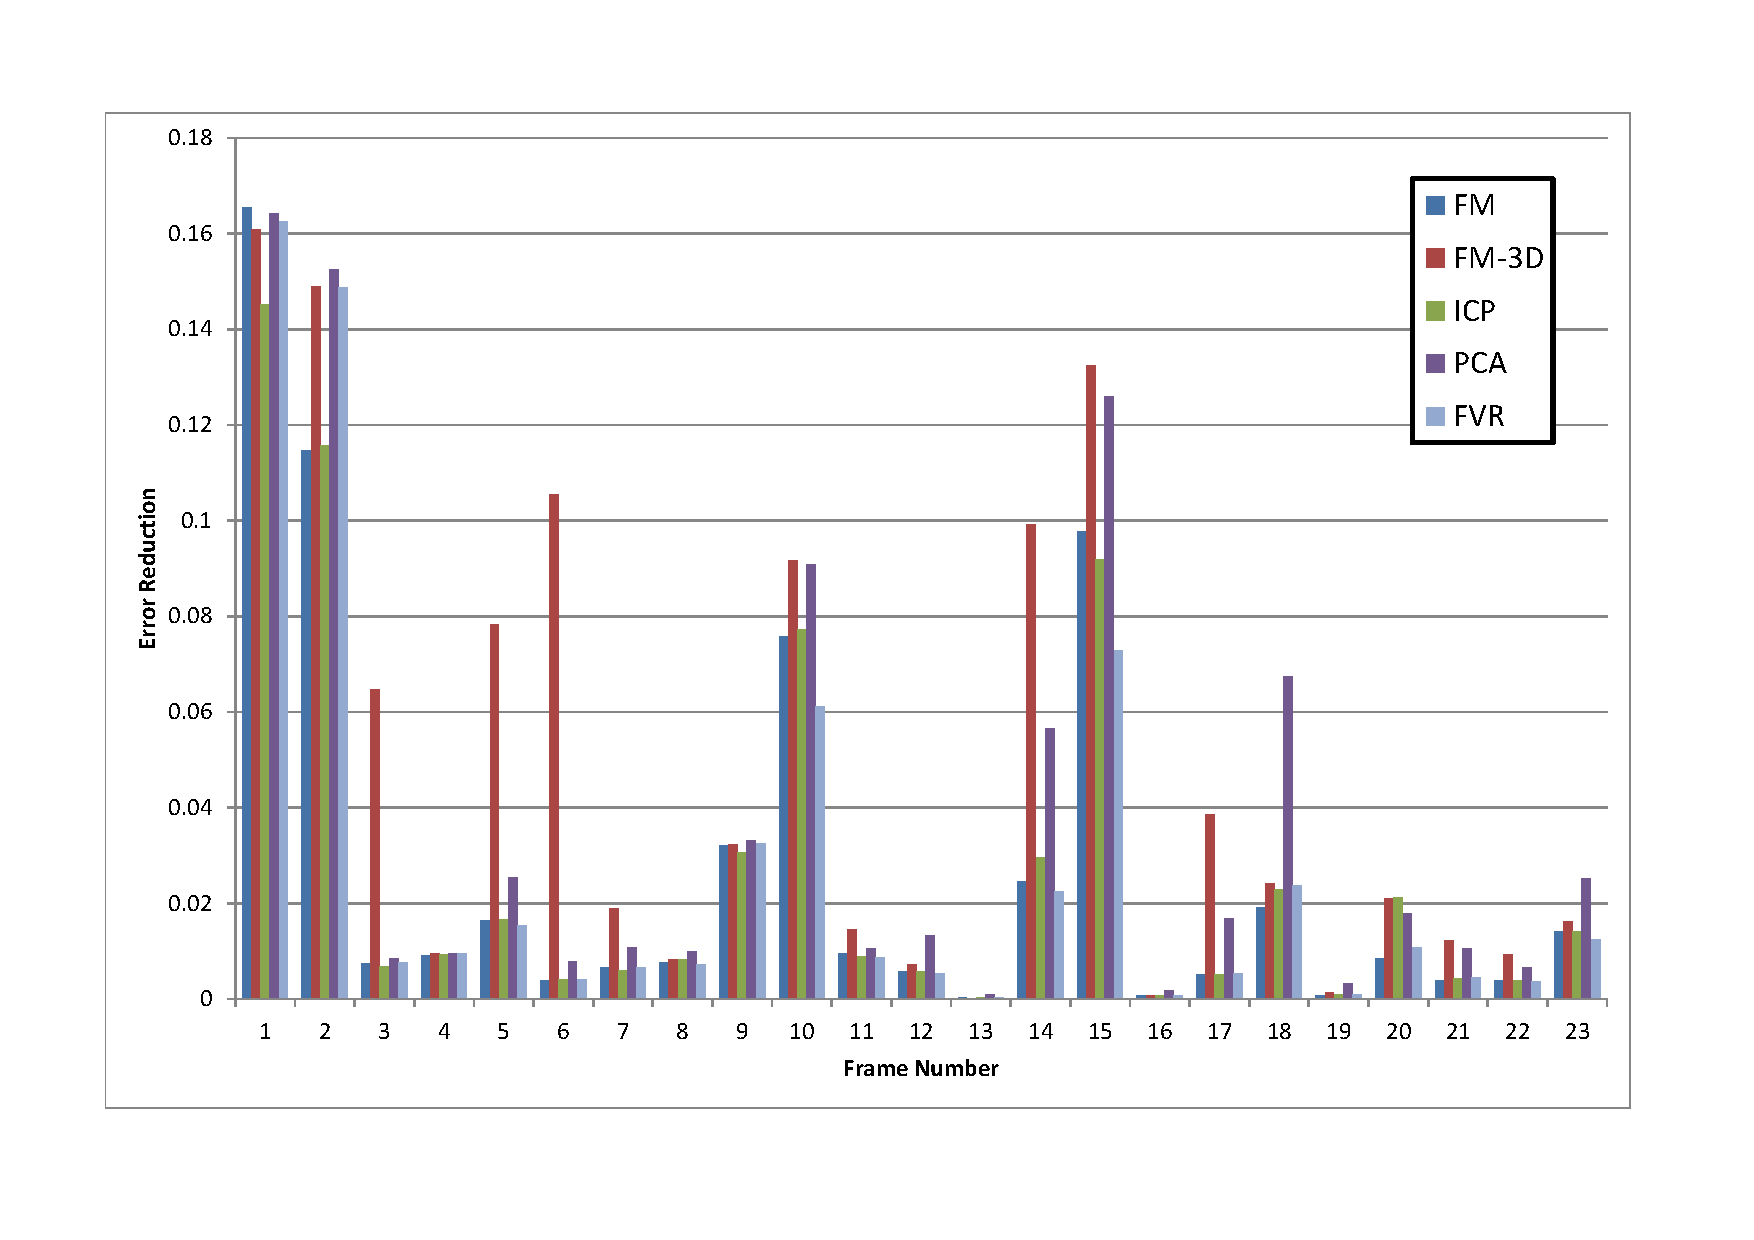
\includegraphics[width=6.0in]{images/results/Apartment_Texture_Rotate}
                \caption{original}
                \label{fig:PEE1}
        \end{subfigure}
       \caption{Registration improvements for Apartment Texture Rotate for different methods.}\label{fig:PEE1Fig}
\end{figure*}

\begin{figure*}[t!] 
        \centering
        \begin{subfigure}[b]{6.0in}
                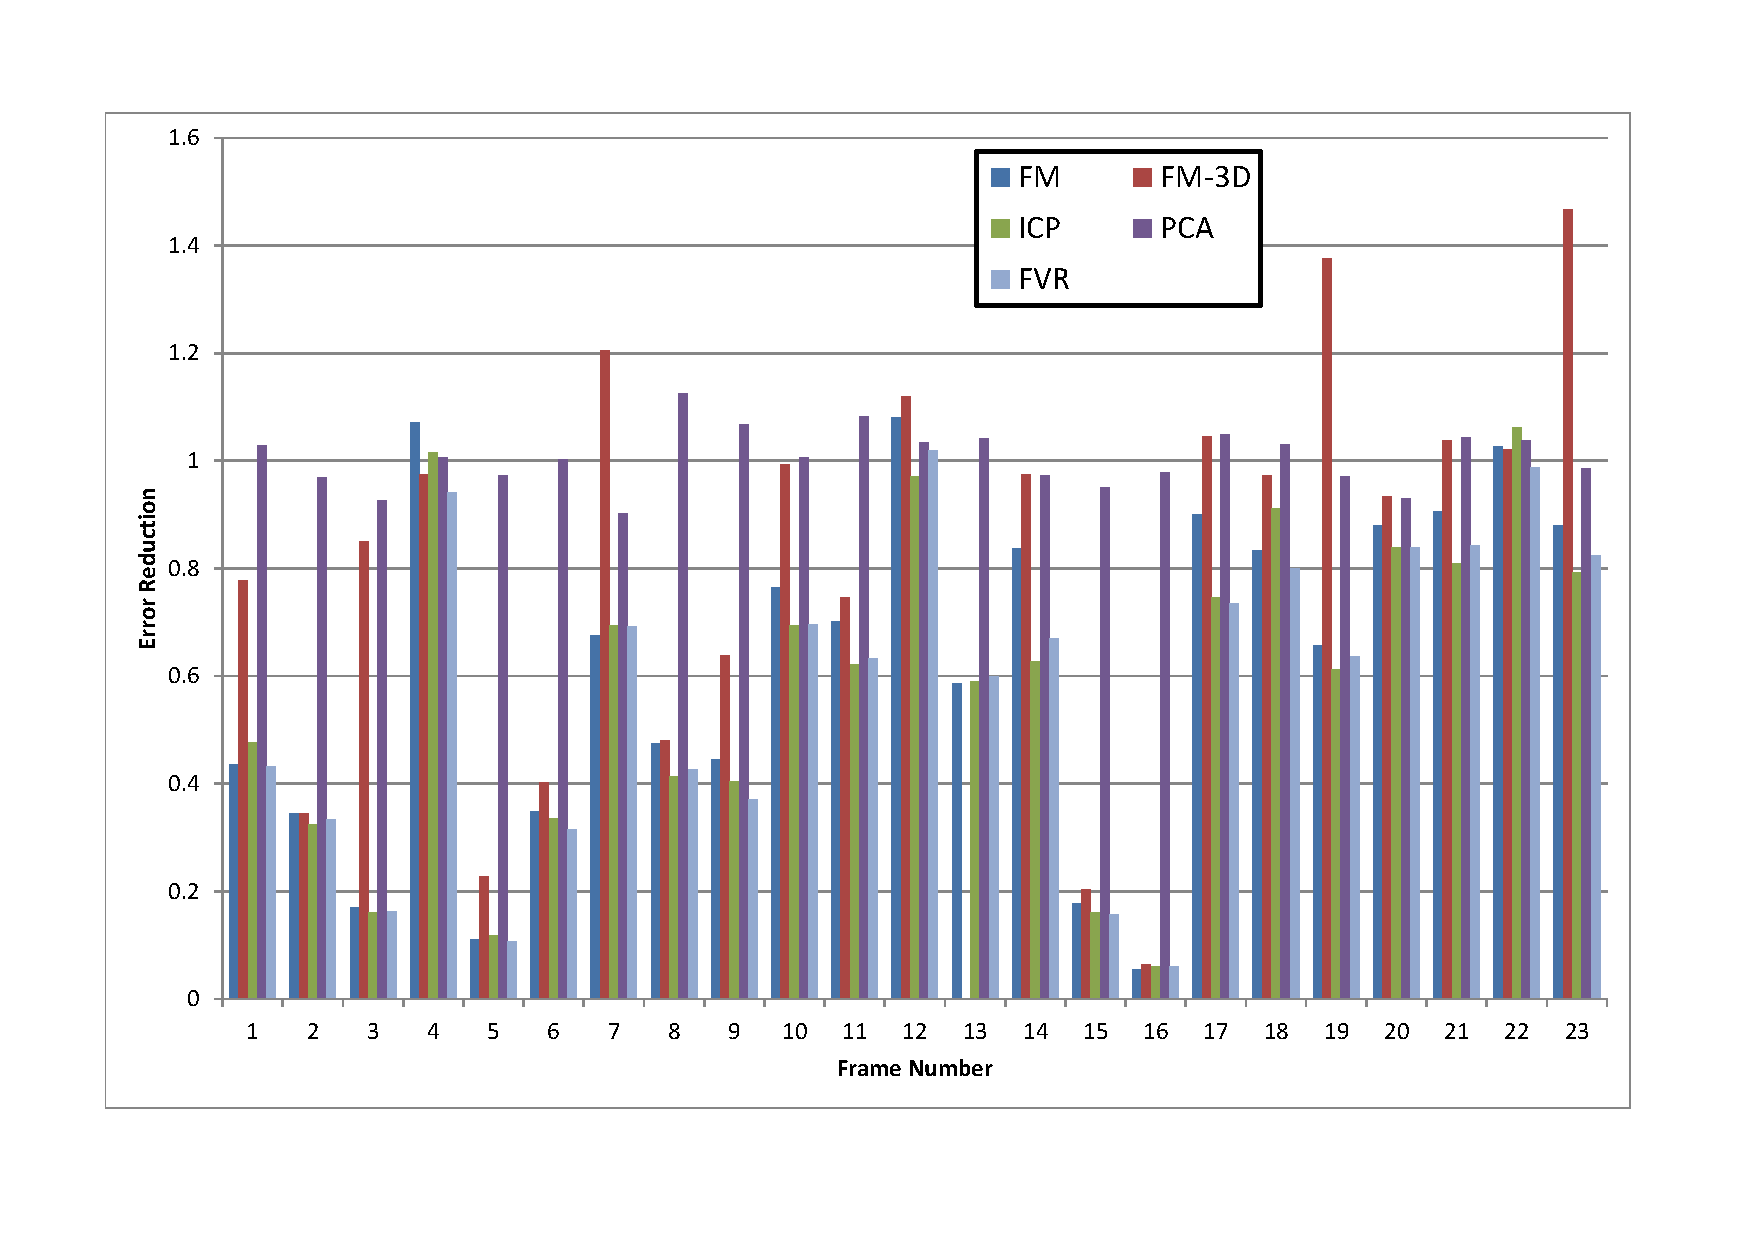
\includegraphics[width=6.0in]{images/results/Apartment_Texture_Rotate_XAxis}
                \caption{original}
                \label{fig:PEE2}
        \end{subfigure}
       \caption{Registration improvements for Apartment Texture X-Axis Rotate for different methods.}\label{fig:PEE2Fig}
\end{figure*}


\begin{figure*}[t!] 
        \centering
        \begin{subfigure}[b]{6.0in}
                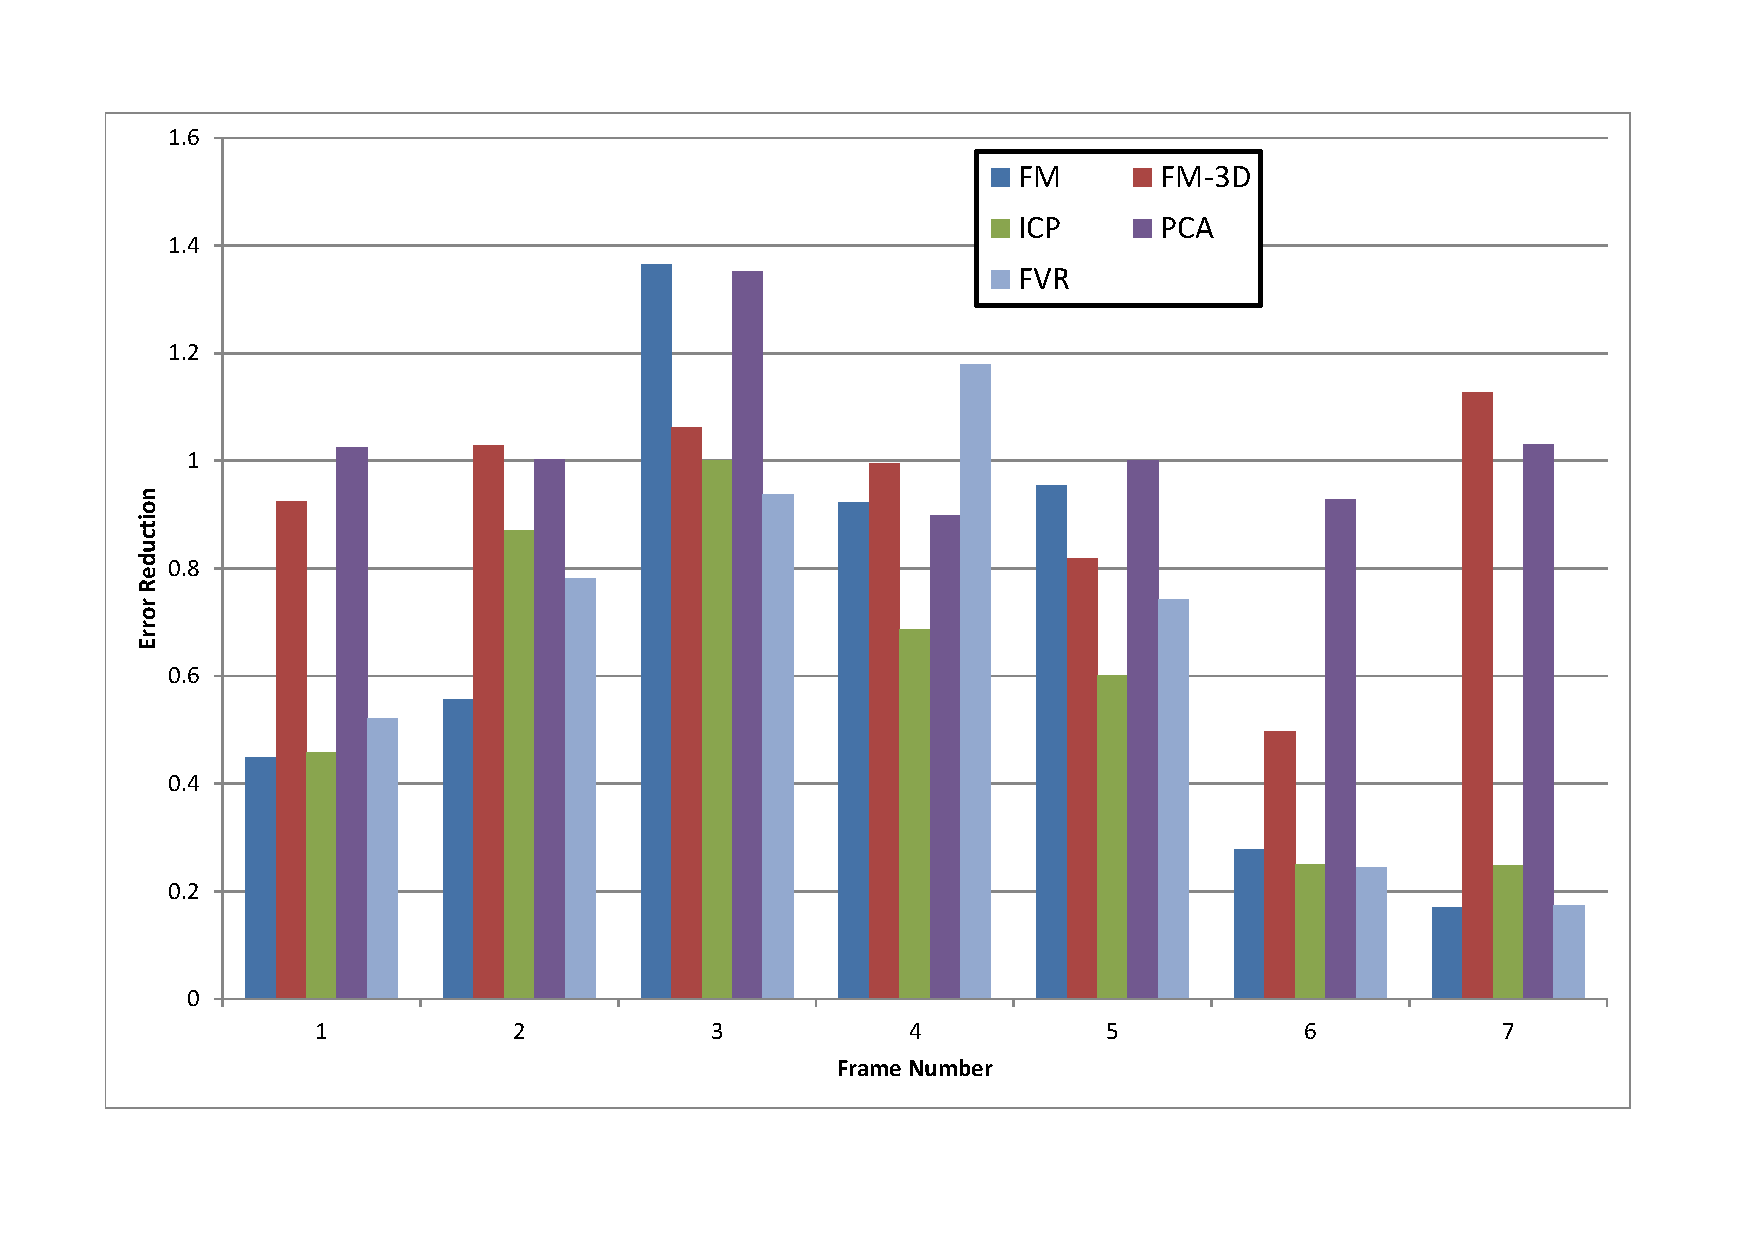
\includegraphics[width=6.0in]{images/results/Boxes_Texture_Rotate}
                \caption{original}
                \label{fig:PEE3}
        \end{subfigure}
       \caption{Registration improvements for Boxes Texture Rotate for different methods.}\label{fig:PEE3Fig}
\end{figure*}

\subsection{3D Registration Experiments}

\subsection{Noise Robustness Tests}

hi


\section{Conclusion}
